\documentclass{article}
\usepackage{ctex}
\usepackage{graphicx} % Required for inserting images
\usepackage{amsmath}
\usepackage{setspace}
\usepackage{indentfirst}
\usepackage{float}
\usepackage[a4paper, left=2cm, right=2cm, top=3cm, bottom=3cm]{geometry}
%\usepackage[backend=biber,style=numeric ]{biblatex}
%\addbibresource{reference.bib}  % 载入参考文献库
\usepackage{url}
\usepackage{appendix}

\title{\zihao{2} \heiti \textbf{Mobile World Congress} 调研报告}
\author{通信四班:张昕}
\date{\today}

\onehalfspacing

\renewcommand{\abstractname}{\zihao{4} 摘要} % 修改摘要标题字号

\setlength{\parindent}{2em}

\begin{document}

\maketitle
\begin{abstract}
{\zihao{-4}
世界移动通信大会(\textbf{英文名}:Mobile World Congress)是世界一年一度的行业大会,由移动通信亚洲大会发起,已经成为全球最具影响力的移动通信领域的展览会,由全球移动通信系统协会主办。本届\textbf{mwc}在西班牙巴塞罗那举行,以“汇聚、连接、创造”为主题,聚焦5G-A,AI、物联网等前沿技术,在这场科技盛宴中,AI与移动通信的深度融合成为核心议题,预示着智能时代的全面崛起。}
\end{abstract}
\section*{AI助力通信}
\zihao{4}
\indent 自\textbf{chatgpt}问世之后,人工智能技术迎来了最近二十年最迅猛的发展时期,\textbf{AI大模型}已经深入我们生活的方方面面。作为全球移动通信的引领者,高通将在\textbf{MWC2025}上展现其前沿技术,高通跃龙\textsuperscript{TM}产品品牌的推出,将覆盖工业及嵌入式物联网、网络和蜂窝基础设施解决方案,赋能众多企业和行业跃上业务新高度。同时,高通FastConnect7700移动连接系统的发布,将加速Wi-Fi7的普及,并将这一前沿技术引入更多主流手机,为用户带来更快的网络速度和更稳定的连接体验。\par
小米作为智能终端领域的佼佼者,此次MWC将展示其“人车家全生态”下的各品类旗舰产品。小米SU7 Ultra、小米15 Ultra等智能手机,以及小米Buds 5 Pro耳机、扫地机器人、智能手表等可穿戴设备和智能家居产品,将全面展现小米在终端AI领域的创新实力和领先地位。\par
\section*{5G-A的创新与发展}
5G-A(5G-Advanced),即5G网络的增强版本,俗称5.5G网络,是今年巴展的一个热词,很多运营商都发布了相关计划,表明从“连接管道”转型为“能力开放平台”、从“以连接(用户)为中心”到“以(用户)体验为中心”的强烈意愿。\par
例如,中国移动和荷兰皇家电信、韩国电信等16家合作伙伴发布了“智能体通信网络白皮书”,中国联通与中国电信联合GSMA(全球移动通信协会)发布了“共享网络智慧共治白皮书”。\par
\begin{figure}[H]
\begin{center}
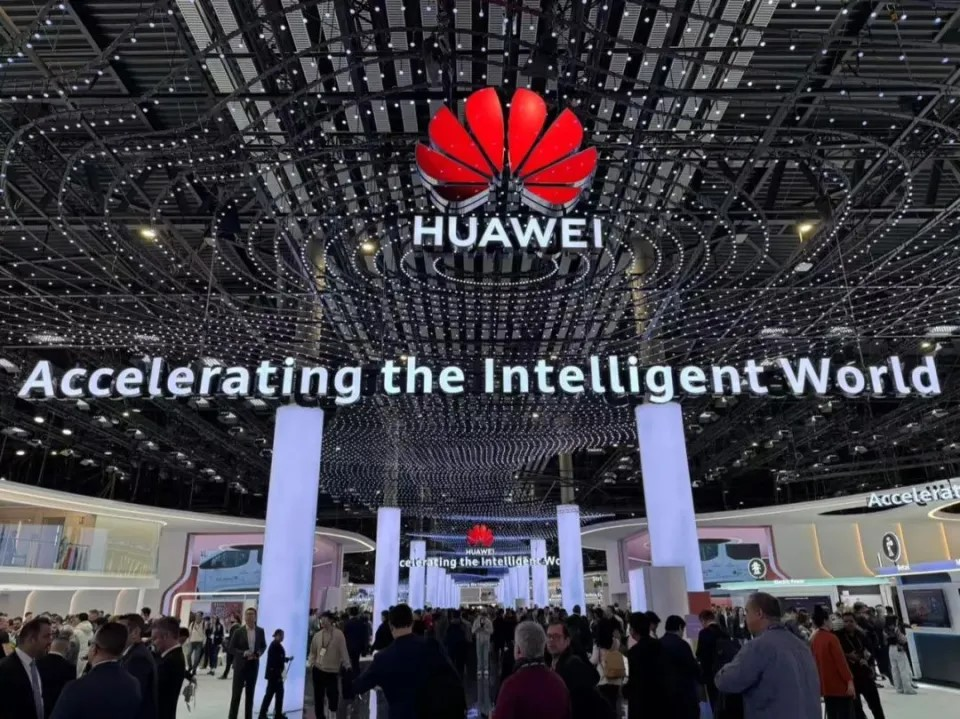
\includegraphics[scale=0.3]{图1}
\caption{\textbf{MWC上的华为展台}}
\end{center}
\end{figure}
相比5G,5G-A不仅有更高速率(上下行传输速度比标准版5G提升10倍)、更广连接、更低时延,还有很多新功能和改进,带来更高的频谱效率、更低的能耗、更强的网络可靠性、安全性,使在线游戏、视频直播、远程医疗手术、自动驾驶、低空飞行、智能制造,以及智能家居和智慧城市等大规模物联网应用,变得更流畅,更高效\cite{news1}\par
\section*{中国力量为世界通信事业发展做出巨大贡献}
在“巴展”开幕前夕,小米在西班牙巴塞罗那召开全球发布会,发布了小米15 Ultra,定价1499欧元,超过了苹果最高端机型iPhone 16 Pro Max的定价。“这样的定价,除了基于不同市场渠道成本、关税等方面的差异考虑外,是小米对自己技术和产品的底气。”卢伟冰说。相比去年的小米14 Ultra,今年小米15 Ultra海外预售的数据增长了100\%以上,其中电商平台12个小时内预售数据已经比去年同期增长了170\%。\par
在中兴展台,宇树科技的四足机器狗、人形机器人进行了现场演示,吸引不少中外参会者拍照。搭载了中兴自研大模型、视觉采集系统的人形机器人能够与中外观众进行中文、日语、英语等多语种对话,听从语音指令握手、行走。在展厅另一边,中兴与天链机器人合作推出的人形机器人Tina也正和参观者互动\cite{news2}。\par
TCL华星的先进显示技术品牌APEX臻图自发布以来备受业界瞩目,它不仅是TCL华星在技术创新路上的重要里程碑,也是将显示技术拓展到应用场景和产业生态的重要一步。本次TCL华星带来的众多展品,将进一步贯彻APEX臻图“洞见极致(PACE TO APEX)”的理念,通过提供更宜人的显示体验、更信赖的视觉健康、更永续的绿色低碳以及更无限的未来想象,为全球消费者带来高品质的视觉感官享受。尤其在当前消费者高度关注的视觉健康领域,TCL华星本次将展出更多具备护眼优势的创新产品。与此同时,TCL华星还将与小米等客户联合展出OLED柔性手机屏幕产品等。TCL华星与小米近年来不断深化合作,对行业前沿半导体显示技术开展预研,从TV到手机、从平板到车载,从联合研发C3 EL材料到C9发光材料,一路推动国产显示技术不断突破\cite{news3}。\par
\begin{figure}[H]
\begin{center}
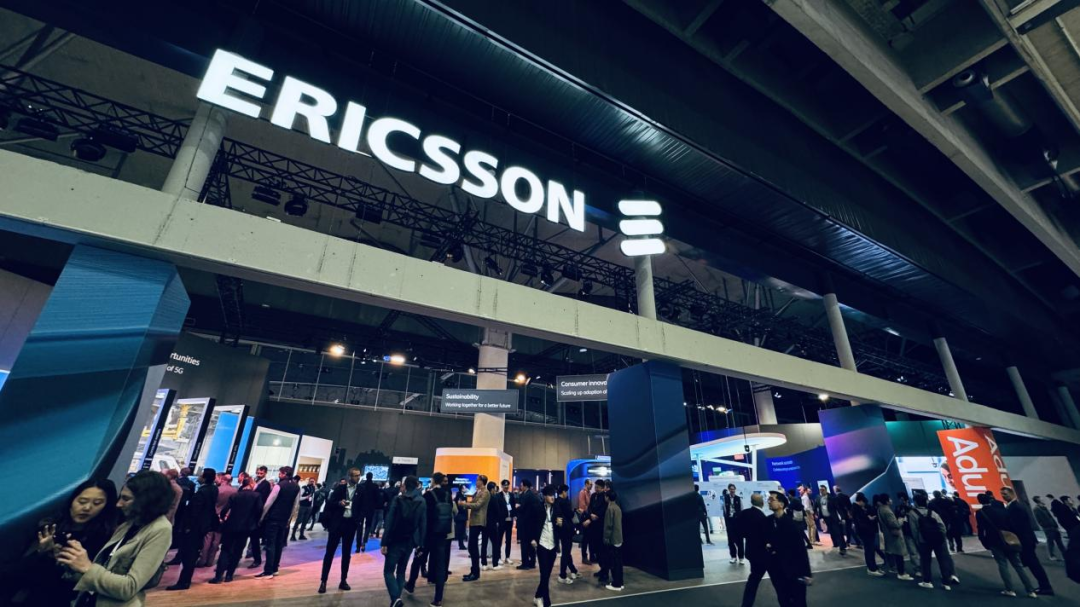
\includegraphics[scale=1]{图2.png}
\caption{爱立信展台}
\end{center}
\end{figure}
\section*{我国移动通信产业的未来与展望}
毋庸置疑,中国自改革开放之后,科学技术产业取得了长足的进步,移动通信领域从无到有,从追赶到反超再到引领,创造了人类历史上的奇迹。但是,展望未来,由于国际形势的不可预估性,以及美国对中国的打压,我们都应该重视发展具有独立自主知识产权的通信技术。\par
对于未来移动通信技术发展的方向,正如在本届巴展开幕主题演讲中,GSMA会长葛瑞德说的,应充分利用AI和开放网关API的潜力,以促进创新和发展\cite{news4}。GSMA在本届巴展期间发布的《2025年移动经济报告》也明确指出,2024年,移动技术和服务贡献了全球GDP的5.8\%(相当于6.5万亿美元的经济价值)。到2030年,这一贡献预计将增至近11万亿美元,占全球GDP的8.4\%。随着5G、物联网和AI等技术的广泛应用,全球生产力和效率将持续提升。\par
\begin{figure}[H]
\begin{center}
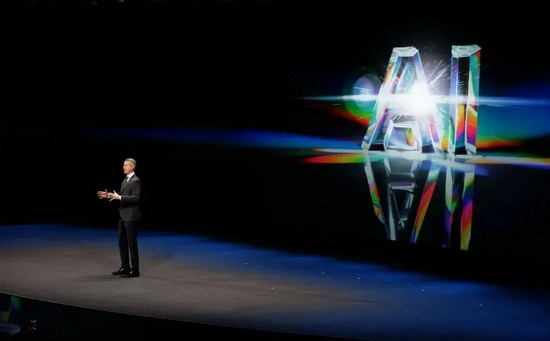
\includegraphics[scale=0.7]{图4.jpg}
\caption{GSMA会长葛瑞德在演讲}
\end{center}
\end{figure}
\section*{总结}
本届世界移动通信大会(MWC2025)充分展现了全球通信技术的最新发展趋势,5G-A、AI、大规模物联网等前沿技术成为行业关注的焦点。大会上,中国企业凭借其卓越的创新能力和产业实力,在智能终端、通信基础设施、显示技术等多个领域展现了领先优势,推动全球通信产业的持续发展。与此同时,全球移动通信行业正朝着更高速率、更低时延、更智能化的方向演进,AI与通信的深度融合也为未来技术升级提供了无限可能。面对国际环境的变化和技术竞争的加剧,中国通信产业需要继续加大自主创新力度,推动核心技术突破,提升产业链自主可控能力,以在未来全球通信格局中保持领先地位。
\newpage
\begin{thebibliography}{9}
    \bibitem{news1} 腾讯新闻. \textit{往前走,莫回呀头——巴展2025所见所想 || 大视野}. 2025年3月10日. \url{https://news.qq.com/rain/a/20250310A004DZ00}
    \bibitem{news2} 新浪财经. \textit{中国科技闪耀“巴展”}. 2025年3月13日. \url{https://finance.sina.com.cn/jjxw/2025-03-13/doc-inepnchr7060880.shtml}
    \bibitem{news3} 新浪财经. \textit{TCL华星即将亮相巴展,共同探索移动通信尖端显示技术}. 2025年2月28日. \url{https://finance.sina.com.cn/cj/2025-02-28/doc-inemzuik9850661.shtml}
    \bibitem{news4} 新浪财经. \textit{巴展回头看:移动AI时代已至}. 2025年3月7日. \url{https://finance.sina.com.cn/tech/roll/2025-03-07/doc-inenvseh9762632.shtml}
\end{thebibliography}
\end{document}